% ═══════════════════════════════════════════════════════════════════════
\section{Pourquoi commencer par là ?}
% ═══════════════════════════════════════════════════════════════════════

\begin{frame}{Pourquoi les transformations, et pourquoi maintenant ?}
  \small
  \begin{itemize}
    \item Ce cours porte sur des mathématiques \textbf{présentes dans la
      technologie} : compression d'images, cryptographie, fractales,
      moteurs de recherche, codes correcteurs.
    \item Les \defi{transformations du plan} sont le premier objet
      mathématique de ce genre --- et le plus visuel.
    \item Une image fractale entière (fougère, triangle de Sierpinski)
      tient dans quelques transformations affines : la figure est ce
      que ces transformations laissent invariant.
  \end{itemize}
  \FigBox[0.36\textheight]{%
    \begin{tikzpicture}[scale=1.5]
      \foreach \ax/\ay in {0/0, 2/0, 1/1.7320508}{
        \foreach \bx/\by in {0/0, 1/0, 0.5/0.8660254}{
          \foreach \cx/\cy in {0/0, 0.5/0, 0.25/0.4330127}{
            \fill[sectioncolor!85]
              ({\ax+\bx+\cx},{\ay+\by+\cy})
              -- ++(0.5,0) -- ++(-0.25,0.4330127) -- cycle;}}}
    \end{tikzpicture}}
  \begin{center}\small Figure 1.1 --- Le triangle de Sierpinski : trois
  transformations affines, dix-huit nombres.\end{center}
\end{frame}

\begin{frame}{Un deuxième motif : le programme du secondaire}
  \begin{itemize}
    \item Les transformations traversent \textbf{tout} le curriculum
      québécois : réflexion (primaire), translation/rotation
      ($1^{\text{re}}$~sec.), homothétie ($2^{\text{e}}$~sec.), langage
      vectoriel ($5^{\text{e}}$~sec.).
    \item Réparties sur plusieurs années, elles sont introduites
      \textbf{une à une}, chacune avec son vocabulaire propre.
    \item L'élève termine avec quatre transformations apprises
      séparément, \textbf{sans avoir vu ce qu'elles ont en commun}.
    \item Cette synthèse n'a pas lieu au secondaire --- mais elle doit
      avoir eu lieu \textbf{chez son enseignant}. C'est l'objet de ce
      chapitre.
  \end{itemize}
\end{frame}

\begin{frame}{Note historique --- le programme d'Erlangen (Klein, 1872)}
  \footnotesize
  \begin{columns}[T]
    \begin{column}{0.27\textwidth}
      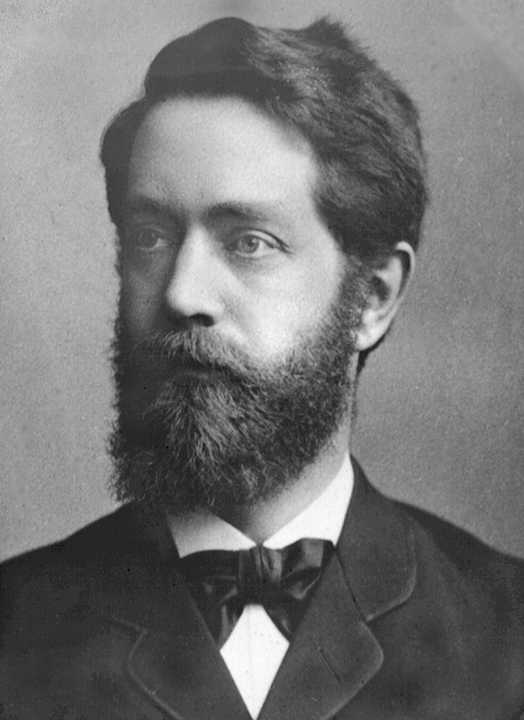
\includegraphics[width=\linewidth]{../../figures/portraits/felix-klein.jpg}\\
      {\scriptsize\color{gray}Felix Klein (1849--1925).}
    \end{column}
    \begin{column}{0.7\textwidth}
      Klein propose de distinguer les géométries non par leurs axiomes,
      mais par leurs \defi{transformations} : l'étude des propriétés
      d'une figure qui restent inchangées sous les transformations
      d'un certain groupe.
      \begin{itemize}
        \item Groupe des \textbf{isométries} : longueurs, angles, aires
          --- géométrie euclidienne du secondaire.
        \item Groupe des \textbf{similitudes} : angles et
          \emph{rapports} de longueurs --- figures semblables.
        \item Groupe des \textbf{transformations affines} : alignement,
          parallélisme, rapports sur une même droite.
        \item Toutes les déformations continues : propriétés
          topologiques seulement.
      \end{itemize}
    \end{column}
  \end{columns}
  \vspace{2pt}
  Plus le groupe est grand, moins on conserve de choses --- mais ce qui
  reste est plus profond. C'est cette hiérarchie qui organise le
  chapitre.
\end{frame}
